\section{Kompressionsverfahren der Feldlinien} \label{konzept}
konzept der unterschiedlichen kompressionsverfahren. zwei lösungsansätze. 
bereits eine simple Kompression implementiert.

\subsection{Ist-Komprimierung} \label{konzept:ist-komprimierung}
\begin{figure}[!htbp]
	\center
	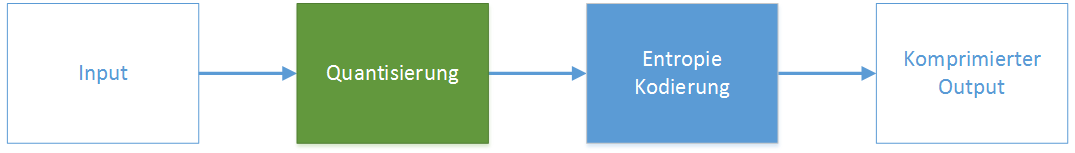
\includegraphics[width=0.8\textwidth,height=6cm,keepaspectratio]{./pictures/konzept/ist/aufbau.png}
	\caption{Aufbau der Ist-Kompression.}
	\label{konzept:ist:aufbau:diagramm}
\end{figure} 
Quantisierung, Formatierung und Kodierung. 
Ist-Kompression. Jeder Kanal wird in 16-Bit Integer quantisiert.
Abspeicherung: Jeder Kanal am Stück, sodass die Entropie Kodierung greifen kann. Entropiekodierung mittels gzip.

Subsampling auf JHelioviewer \ref{konzept:loesung0:subsampling}

Der JHelioviewer bietet an, die Feldlinien zu einem gegebenen Zeitpunkt darzustellen. Damit der Benutzer eine vernünftige Zeit auf die Feldlinien wartet, wurde bereits im Vorfeld eine Kompression implementiert. Zuerst werden die Daten im sphärischen Koordinatensystem(Radius, Längengrad $\phi$ und Breitengrad $\theta$) auf dem Server quantisiert und mit GZip verlustfrei komprimiert. Der JHelioviewer dekomprimiert die Daten und transformiert sie in das kartesische Koordinatensystem um. Die Punktmenge wäre für schwächere Grafikkarten zu gross, weshalb der JHelioviewer eine weitere Quantisierung durchführt.\\

\textbf{Quantisierung und Dateiformat auf dem Server}\\
Zuerst werden die Kanäle R,$\phi$ und $\theta$ Kanäle zu shorts diskretisiert:
\begin{enumerate}
 \item R: 4 = $2^{15}$. 
 \item $\phi$: $2\pi$ = $2^{15}$
 \item $\theta$: $2\pi$ = $2^{15}$
\end{enumerate}
$\theta$ Wertebereich geht aber nur von 0 bis $\pi$, die letzten Bits werden gar nicht verwendet. Die Kanäle R und $\phi$ haben das Problem, dass der Wert $2^{15}$ einen Signed Integer Overflow verursacht und auf $-2^{15}$ zu liegen kommt. R scheint den maximalen Wert nie zu erreichen. Wenn aber eine Feldlinie den Nullpunkt passiert, springt der Kanal von  $2^{15}-1$ auf $-2^{15}$ und dann auf 0.\\
[\baselineskip]
Subsampling, jeder vierte Punkt 
0 Löschen.

Format: zuerst Konstanten, alle Radien\\

\textbf{Quantisierung des JHelioviewers}\\
Clientseitig wieder ein subsampling und umrechnung ins kartesische System xyz, dann Anglesubsampling
	
\subsection{Lösungsansatz Adaptives Subsampling}
\begin{figure}[!htbp]
	\center
	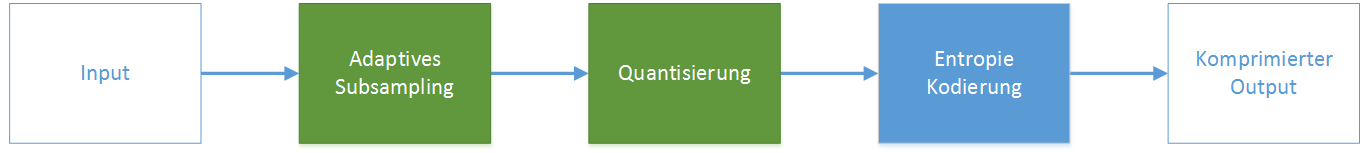
\includegraphics[width=0.8\textwidth,height=6cm,keepaspectratio]{./pictures/konzept/solution0/aufbau.png}
	\caption{Aufbau des Lösungsansatzes: Adaptives Subsampling.}
	\label{konzept:loesung0:aufbau:diagramm}
\end{figure} 
Subsampling wird nun auf dem Server ausgeführt. in den folgenden Abschnitten sind die Teilschritte erklärt.

\subsubsection{Adaptives Subsampling}\label{konzept:loesung0:subsampling}
Ziel des adaptiven Subsamplings ist es, die Daten durch eine Folge von Strecken zu approximieren. An stellen, welche die Feldlinie gekrümmt ist, braucht es mehr Strecken. An Stellen, welche die Feldlinie Linear verlauft können so viele Punkte gespart werden. 
\begin{figure}[!htbp]
	\center
	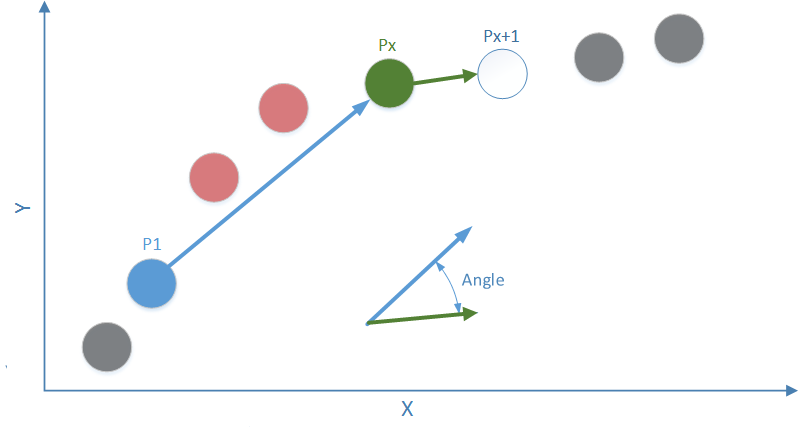
\includegraphics[width=0.8\textwidth,height=6cm,keepaspectratio]{./pictures/konzept/solution0/anglesubsampling.png}
	\caption{Darstellung des Adaptiven Subsapmlings im 2D Raum.}
	\label{konzept:loesung0:angle}
\end{figure}
Das Diagramm der Abbildung \ref{konzept:loesung0:angle} stellt das Subsampling im zweidimensionalen Raum dar. Zu sehen sind die Punkte der Feldlinie. Das Adaptive Subsampling wählt nun Punkte $P$ aus der Feldlinie aus, welche Start- und Endpunkte der Strecken darstellen.\\
$P_1$ wurde bereits ausgewählt. Es wird nun ein Punkt $P_x$ gesucht, der als Endpunkt einer Strecke von $P_1$ zu $P_x$ die Feldlinie approximiert. Dazu wird der Winkel der Strecke $P_1$ zu $P_x$ mit der Strecke $P_x$ zu $P_x+1$ verglichen. Wenn der Winkel kleiner ist, als ein Faktor $F$, wird der nächste Punkt $P_x+1$ überprüft. Wenn der Winkel grösser ist, wird $P_x$ ausgewählt und von $P_x$ aus weiter geprüft.

\subsubsection{Entropie Kodierung} \label{konzept:loesung0:kodierung}
Abspeicherung, Alle X Kanäle hintereinander, alle Y Kanäle etc. So kann die Entropide-Kodierung besser greifen.
Rar hat sich bewährt bei der purer Feldlinien kompression im Vergleich zu anderen Verfahren wie LZ77/gZip. Bringt etwa 4 mal bessere Kompression hin, hat aber mehr mühe mit Floating-Point nummern als mit Integers

\subsection{Lösung 1, Diskrete Kosinus Transformation}
Bild
DCT, da alles nahe an harmonischen Halbwellen
kartesische Koordinaten --> kein wrap around,

Es ist auch möglich die Punkte im sphärischen Koordinatensystem in den Frequenzraum zu überführen. Der $\phi$-Kanal ist jedoch schwierig durch tiefe Kosinus Schwingungen darzustellen: Wie im Abschnitt \ref{konzept:ist-komprimierung} besprochen, beinhaltet der Kanal Sprünge bei der Passierung des Nullpunktes. Das führt zu sehr hochfrequenten Schwingungsanteile in der DCT. Nach einer Quantisierung sind dabei Artefakte nicht vermeidbar. Im kartesischen System hingegen sind alle Kanäle stetig und lassen sich einfacher durch Kosinus-Funktionen approximieren.\\

\subsubsection{Subsampling} \label{konzept:loesung1:subsampling}
Wie im Abschnitt \ref{testsetup:auswahl_erhebung} beschrieben, wurde aus den Testdaten die Quantisierung und das Subsampling entfernt. Die Feldlinien der Testdaten haben das vier Mal mehr Puntke, als beim Ist-Zustand übertragen werden. Die DCT-Implementierung weist eine Komplexität von $O(n^2)$ auf. Vor der Kosinus-Transformation wird deshalb das selbe Subsampling durchgeführt, wie im Ist-Zustand. So kann der Rechenaufwand in Grenzen gehalten werden.\\
Falls die Laufzeit der Dekompression verbessert werden soll, kann die Fast-Cosine-Transformation umgesetzt werden. Diese hat eine Komplexität von $O(n log(n))$. Der Nachteil ist, dass nur Daten der Länge $2^n$ transformiert werden können, was zusätzliche Programmlogik braucht. Falls die Fast-Cosine-Transformation nicht ausreicht, können die Linien in Blöcken mit einer bestimmten Anzahl von Punkten unterteilt werden. Dadurch wird die Komplexität auf $O(n)$ gesenkt. Jedoch ist es wahrscheinlich, dass durch die Unterteilung die Kompressionsrate leidet. Vermutlich braucht es für die Approximation der Blöcke insgesamt mehr Kosinus-Funktionen, als für die Approximation der gesamten Feldlinie.\\

\subsubsection{Randbehandlung} \label{konzept:loesung1:randbehandlung}

\subsubsection{Cosinus-Transformation} \label{konzept:loesung1:kosinus}
Transformiert Daten in den Frequenzraum. Eine Menge von Punkten mit der Länge $N$ kann in eine Menge von $N$ Kosinusfunktionen überführt werden.\\
Es gibt verschiedene Möglichkeiten die Punkte zu transformieren. Der Unterschied liegt in der RAndbehandlung. Es wurde sich am JPEG/JFIF Standard orientiert(cite JPEG paper 1997), welcher, welche die DCT-II als Forwärts und die DCT-III als Rückwärtstransformation verwendet.
Der Rand
$X_k = \sum_{n=0}^{N-1}x_n cos[\frac{\pi}{N}(n+\frac{1}{2}k)]
 k= 0,1,\ldots,N-1$
$N$ ist anzahl Punkte. Transformiert in den Frequenzraum. $x_n$ ist ein Punkt des Signales und $X_k$ ist die Resultierende Kosinus Schwingung%? wirklich schwingung oder was anderes?

Inverse Transform
$X_k = \frac{1}{2}x_0 + \sum_{n=1}^{N-1}x_n cos[\frac{\pi}{N}n(k+\frac{1}{2}]  k= 0,1,\ldots,N-1$

\subsubsection{Quantisierung}

\subsubsection{Ablegung ins Fits Format}

\subsubsection{Entropie Kodierung}\label{konzept:loesung1:kodierung}
Kodierung
	Zuerst einfaches Run-length

	Weitere Kodierung mittels Rar.
		Rar hat sich bewährt bei der purer Feldlinien kompression im Vergleich zu anderen Verfahren wie LZ77/gZip





